
\section{Instruction set architectures}
An Instruction Set Architecture (ISA) specifies the syntax and semantics of the
assembly language on each architecture. It is not just a different syntax but
is built in the core design of a processor, as it affects the way and order
instructions are executed and their level of complexity. ISA mainly consists of
the following components:

\begin{itemize}
    \item  Instructions: the instruction to be processed in the {\bf opcode
        operand\_list format}. There are usually 1,2, or 3 comma-separated
    operands \verb+add rax, 1+ \ldots)
    \item  Registers: Used to store operands, addresses, or instructions
        temporarily (\verb+rax, rsp, rip+)
    \item  Memory Addresses: The address in which data or instructions are
        stored. May point to memory or registers 
        (\verb+0xffffffffaa8a25ff, 0x44d0, $rax+)
    \item  Data Types:  The type of stored data (byte, word,\ldots).
\end{itemize}

These are the main components that distinguish different ISA's and assembly languages. 

There are two main Instruction Set Architectures that are widely used:

\begin{itemize}
    \item Complex Instruction Set Computer (CISC) - Used in Intel and AMD
        processors in most computers and servers.
    \item Reduced Instruction Set Computer (RISC) - Used in ARM and Apple
        processors, in most smartphones, and some modern laptops.
\end{itemize}

Let us see the pros and cons of each and the main differences between them.

\subsection{CISC}

The CISC architecture was one of the earliest ISA's ever developed. As its name
suggests, the CISC architecture favors more complex instructions to be run at a
time to reduce the overall number of instructions. This is done to rely as much
as possible on the CPU by combining minor instructions into more complex
instructions.

For example, suppose we were to add two registers with the \verb+add rax, rbx+
instruction. In that case, a CISC processor can do this in a single
'Fetch-Decode-Execute-Store' instruction cycle, without having to split it into
multiple instructions to fetch \verb+rax+, then fetch \verb+rbx+, then add
them, and then store them in `rax, each of which would take its own
'Fetch-Decode-Execute-Store' instruction cycle.

Two main reasons drove this:
\begin{itemize}
    \item To enable more instructions to be executed at once by designing the
        processor to run more advanced instructions in its core.
    \item In the past, memory and transistors were limited, so it was preferred
        to write shorter programs by combining multiple instructions into one.
\end{itemize}

To enable the processors to execute complex instructions, the processor's
design becomes more complicated, as it is designed to execute a vast amount of
different complex instructions, each of which has its own unit to execute it.

Furthermore, even though it takes a single instruction cycle to execute a
single instruction, as the instructions are more complex, each instruction
cycle takes more clock cycles. This fact leads to more power consumption and
heat to execute each instruction.

\subsection{RISC}

The RISC architecture favors splitting instructions into minor instructions,
and so the CPU is designed only to handle simple instructions. This is done to
relay the optimization to the software by writing the most optimized assembly
code.

For example, the same previous \verb+add r1, r2, r3+ instruction on a RISC
processor would fetch \verb+r2+, then fetch \verb+r3+, add them, and finally
store them in \verb+r1+. Every instruction of these takes an entire
'Fetch-Decode-Execute-Store' instruction cycle, which leads, as can be
expected, to a larger number of total instructions per program, and hence a
longer assembly code.

By not supporting various types of complex instructions, RISC processors only
support a limited number of instructions (~200) compared to CISC processors
(~1500). So, to execute complex instructions, this has to be done through a
combination of minor instructions through Assembly.

On the other hand, an advantage of splitting complex instructions into minor
ones is having all instructions of the same length either 32-bit or 64-bit
long. This enables designing the CPU clock speed around the instruction length
so that executing each stage in the instruction cycle would always take
precisely one machine clock cycle.

The below diagram shows how CISC instructions take a variable amount of clock
cycles, while RISC instructions take a fixed amount: risc vs cisc cycles



 \begin{figure}
  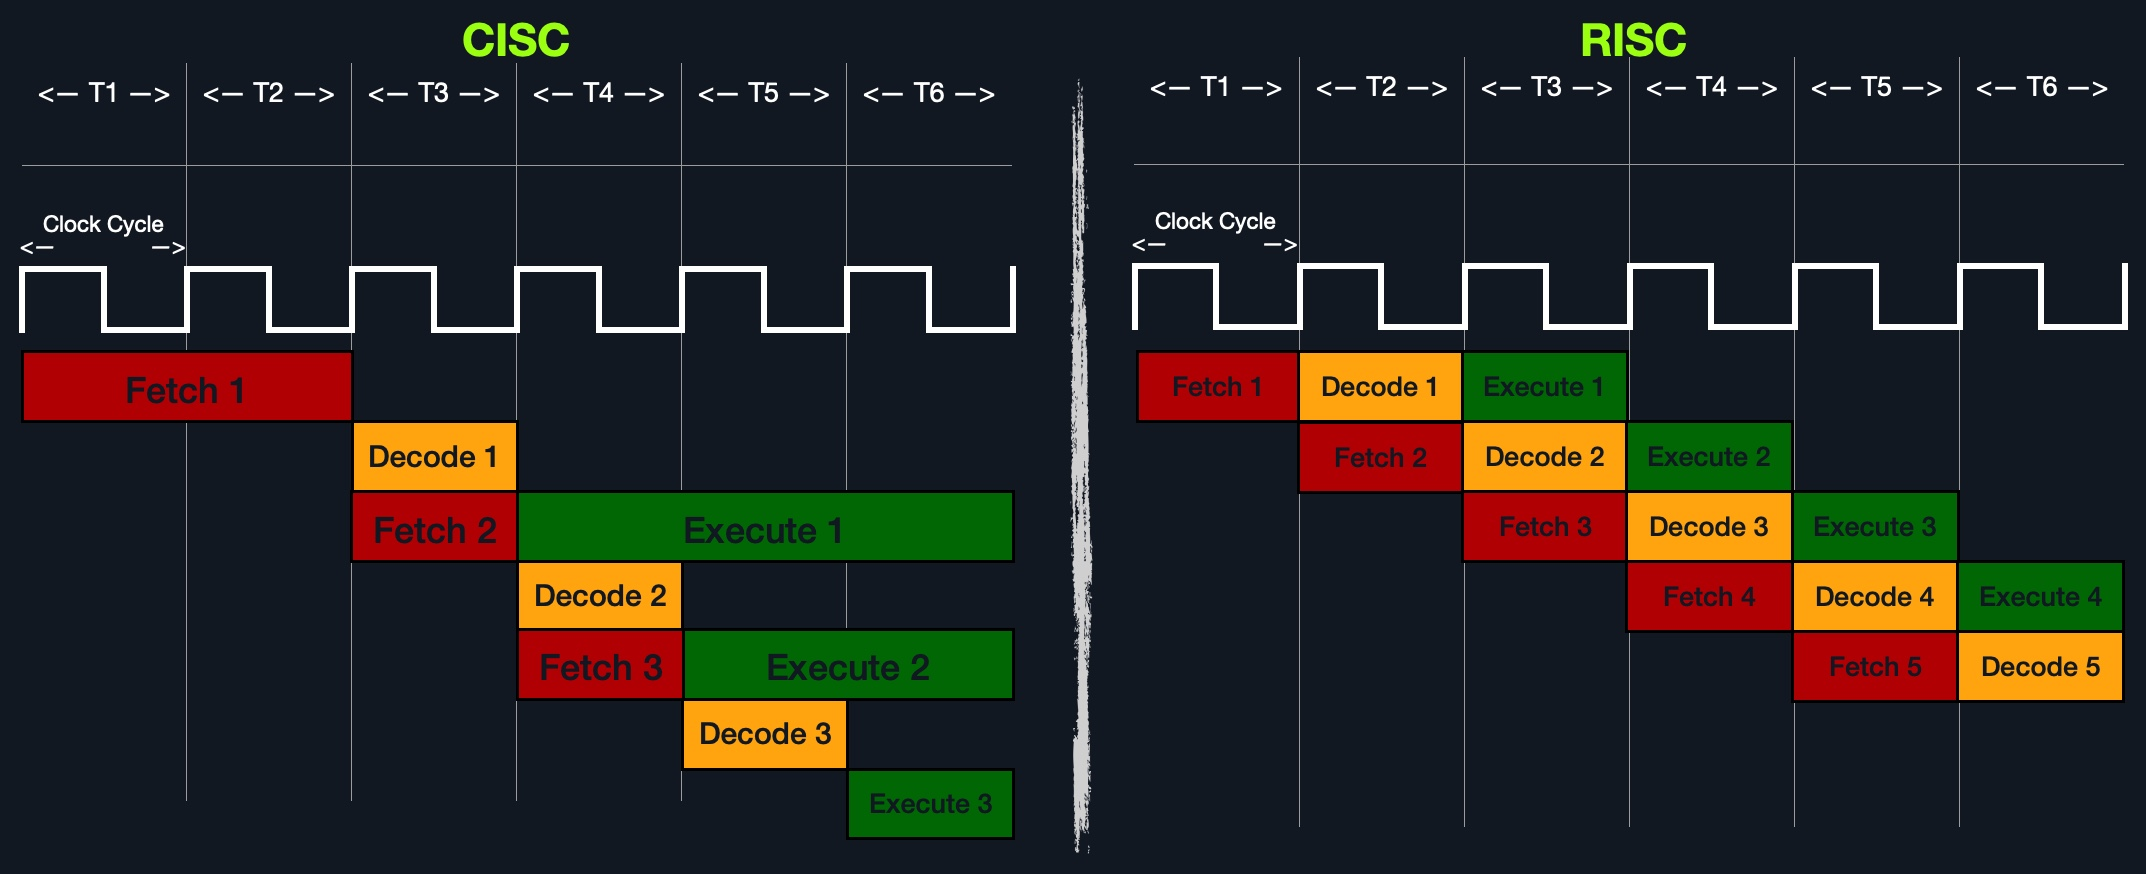
\includegraphics[width=\linewidth]{binary/intro/images/assembly_cisc_risk_cycles.jpg}
  \caption{CISC / RISC cycles}
  \label{fig:assembly_cisc_risk_cycles}
\end{figure}



Executing each instruction stage in a single clock cycle and only executing
simple instructions leads to RISC processors consuming a fraction of the power
consumed by CISC processors, which makes these processors ideal for devices
that run on batteries, like smartphones and laptops.

\subsection{CISC vs. RISC}
In the past, having a longer assembly code due to a larger number of total
instructions per program was a significant disadvantage for RISC processors due
to the limited resources in memory and storage. However, today this is no
longer as big of an issue, as memory and storage are not as expensive and
limited as they used to be in the past.

Furthermore, with new assemblers and compilers writing extremely optimized code
on the software level, RISC processors are becoming faster than CISC
processors, even in executing and processing heavy applications, all while
consuming much less power.

All of this is making RISC processors more common in recent years. RISC may
become the dominant architecture in the upcoming years. But as we speak, the
overwhelming majority of computers and servers we will be pentesting are
running on Intel/AMD processors with the CISC architecture, making learning
CISC assembly our priority. As the basics of all Assembly language variants are
pretty similar, learning ARM Assembly should be more straightforward.



